\documentclass[times,twocolumn,final]{elsarticle}
\usepackage{cag}
\usepackage{framed,multirow}
\usepackage{amssymb}
\usepackage{amsmath}
\usepackage{lineno}
\usepackage{graphicx}
\usepackage{url}
\usepackage{booktabs}
\usepackage{placeins}
\usepackage{array}
\graphicspath{{../figures/}{figures/}}
\setlength{\emergencystretch}{2em}
\setlength{\hfuzz}{2pt}
\setcounter{totalnumber}{6}
\setcounter{topnumber}{4}
\setcounter{bottomnumber}{4}
\renewcommand{\topfraction}{0.92}
\renewcommand{\textfraction}{0.05}
\renewcommand{\floatpagefraction}{0.85}
\journal{Computers \& Graphics}
\begin{document}
\begin{frontmatter}

\title{Measured Effects and Limits of Inference-Time Geometry-Adapter Scaling for Multi-view Texture Generation}

% Double-anonymous review: author names, affiliations, and acknowledgements
% are supplied separately after the scientific and editorial gates close.

\begin{abstract}
Geometry-conditioned multi-view diffusion pipelines commonly expose an adapter scale as a single inference-time control. Its numerical value, however, does not fully specify the intervention: per-layer caps, temporal placement, and the adapter's residual path determine the applied scale and realized correction. We report a bounded empirical study of these effects in an MVPainter-style texture-generation pipeline. On a disjoint 150-object cohort whose analysis safeguards followed prior outcome exposure, a late-high profile (LLH) differs from an exact per-layer-mean constant profile by +0.325 dB in foreground PSNR (95\% object-bootstrap CI [0.209, 0.446]) and -0.00460 in foreground LPIPS ([-0.00563, -0.00357]); both intervals fall inside predeclared practical margins. Against an equal-high-duration early-high profile, the mean PSNR difference is positive but heterogeneous: 45.3\% of objects favor LLH and the median difference is negative, while LPIPS favors LLH on 80.7\% of objects. A fixed-cohort three-seed sensitivity and static 2\,$\times$\,2 scale analysis show additional profile-specific responses, but do not identify a dose-independent layer-by-time law. A sampler-conformant evaluation of stored GLBs (20 UV-supported objects, 11 unseen views) yields mixed endpoint directions and does not establish overall 3D fidelity. We therefore present no universal schedule, unique winner, human-preference claim for LLH, seam claim, or cross-backbone transfer law. The contribution is a reproducible characterization of the tested residual/cap semantics and their object-, metric-, and interface-specific limits; its methodological novelty remains bounded by recent layer/time scheduling prior work.
\end{abstract}

\begin{keyword}
\KWD
multi-view diffusion \sep 3D texture generation \sep adapter scaling \sep residual dose \sep empirical evaluation
\end{keyword}

\end{frontmatter}
\linenumbers

\section{Introduction}
\label{sec:intro}

Geometry-conditioned diffusion is widely used to generate multi-view images for 3D texturing. Systems such as MVPainter inject geometric information through a learned adapter and then project or bake generated views onto a mesh \cite{shao2025mvpainter}. At inference time, a scale controls the adapter contribution. A scalar label is convenient, but it can conceal where the residual is injected, whether implementation caps activate, and how large the post-scale correction is. Two profiles with the same requested scale integral need not apply the same scales or produce the same residual norms.

A second issue is evidential. Higher PSNR, structural similarity, or texture-variation statistics do not by themselves establish faithful material reproduction. A generated surface can have strong high-frequency response and still contain color shifts, repeated patterns, or missing detail. Likewise, an average paired difference can be statistically precise while being small relative to a practical margin or heterogeneous across objects. These distinctions matter for a method whose stated purpose is to balance geometry adherence and texture appearance.

The broad operation of scheduling diffusion controls across network depth and denoising time is not new. Scheduled Style Injection studies layer- and timestep-varying parameters for training-free style transfer and also evaluates schedules for geometric ControlNet conditioning \cite{kulkarni2026scheduled}. Its task and intervention differ from the MVPainter residual path studied here, but this overlap rules out a general claim that layer-by-time control is itself a new diffusion mechanism. We instead ask a narrower question: what can paired evidence establish about specified scale profiles, caps, realized residual dose, object heterogeneity, and output endpoints in this geometry-conditioned texture pipeline?

Our evidence supports a bounded answer. On the fresh object cohort, LLH is not a universal winner. Its difference from an exact layer-mean constant profile is statistically detectable but inside prespecified practical margins; its mean PSNR advantage over HLL is not typical of most objects; and a generic linear schedule is competitive or better on some endpoints. A static scale factorial detects layer-group sensitivity on a reused subset, but does not vary time or equalize realized dose. In the 3D endpoint, LLH improves LPIPS relative to the native fixed-low profile while PSNR and CIEDE2000 do not support an overall advantage. Results on MV-Adapter and MVDiffusion further bound transfer without identifying an architecture-caused difference.

The paper makes four contributions. First, it defines a reproducible distinction among requested scale, cap-applied scale, and measured post-scale residual norm. Second, it reports object-paired estimates and practical margins for four schedule contrasts, separating registered comparisons from an exploratory contrast. Third, it provides bounded realization and static-scale sensitivity analyses with their reused-cohort limitations. Fourth, it reports the supported GLB-native endpoint and separate interface-specific results, while withdrawing claims of human-validated fidelity, seam improvement, unique optimality, dose-independent interaction, and broad transfer.

\section{Related work and contribution scope}
\label{sec:related}

\subsection{Geometry-conditioned multi-view texture generation}

MVPainter and related systems use multi-view diffusion and geometric conditions to synthesize texture views for 3D assets \cite{shao2025mvpainter}. ControlNet and adapter methods provide learned pathways for adding spatial conditions to diffusion models \cite{zhang2023controlnet}. MV-Adapter uses a distinct multi-view adapter architecture \cite{huang2025mvadapter}; MVDiffusion instead uses correspondence-aware attention for joint multi-view generation \cite{tang2023mvdiffusion}. These interfaces do not expose an interchangeable residual variable, so comparisons across them must remain within each tested pipeline.

\subsection{Inference-time schedules and prior art}

Diffusion guidance and condition strength have been varied over denoising steps, including limited-interval classifier-free guidance \cite{kynkaanniemi2024limited}. Scheduled Style Injection is the closest prior work for the present framing: it schedules StyleID parameters across decoder depth and time and also studies geometric ControlNet scale on both axes \cite{kulkarni2026scheduled}. Consequently, this paper does not claim novelty for training-free scheduling, the layer/time axes, or the general idea of changing control strength over denoising. The domain-specific evidence here concerns one MVPainter-style residual path, explicit per-layer caps and measured correction norms, object-level paired texture metrics, and a bounded baked-texture endpoint. Whether this empirical scope is sufficiently substantial for the target venue remains an editorial question, not a result established by the experiments.

\subsection{Image and appearance metrics}

We report PSNR and SSIM-type measures as reference and structural comparisons, and LPIPS as a learned feature-distance measure \cite{wang2004ssim,zhang2018lpips}. These are complementary image-space endpoints, not direct measurements of perceived material identity. Laplacian variance, color spread, gradient magnitude, and high-frequency energy are treated as variation diagnostics only. They can increase because of artifacts as well as detail; none is used as a stand-alone fidelity criterion.

\section{Intervention and study design}
\label{sec:method}

\subsection{Requested scale, caps, and realized residual dose}

At layer group $\ell$ and denoising step $t$, let $r_{\ell,t}$ be the adapter correction before the external scale. The requested scale is $s^{\mathrm{req}}_{\ell,t}$. On the native capped path, the applied scale is
\begin{equation}
 s^{\mathrm{app}}_{\ell,t}=\min(s^{\mathrm{req}}_{\ell,t},c_\ell),\qquad
 \Delta h_{\ell,t}=s^{\mathrm{app}}_{\ell,t}r_{\ell,t},
\end{equation}
where $c_\ell$ is the implementation cap. The tested caps are 3.0 (deep), 3.5 (middle), and 0.8 (shallow). A requested-scale integral $D_\ell=\sum_t s^{\mathrm{req}}_{\ell,t}$ describes the control request, not its realized effect. We separately record the per-object post-scale correction norm
\begin{equation}
 E_{i,\ell}=\left(\sum_t\|\Delta h_{i,\ell,t}\|_2^2\right)^{1/2}.
\end{equation}
Neither $D_\ell$ nor $E_{i,\ell}$ captures residual direction or all nonlinear downstream interactions. We therefore do not interpret either as a complete causal dose measure.

\begin{figure*}[t]
\centering
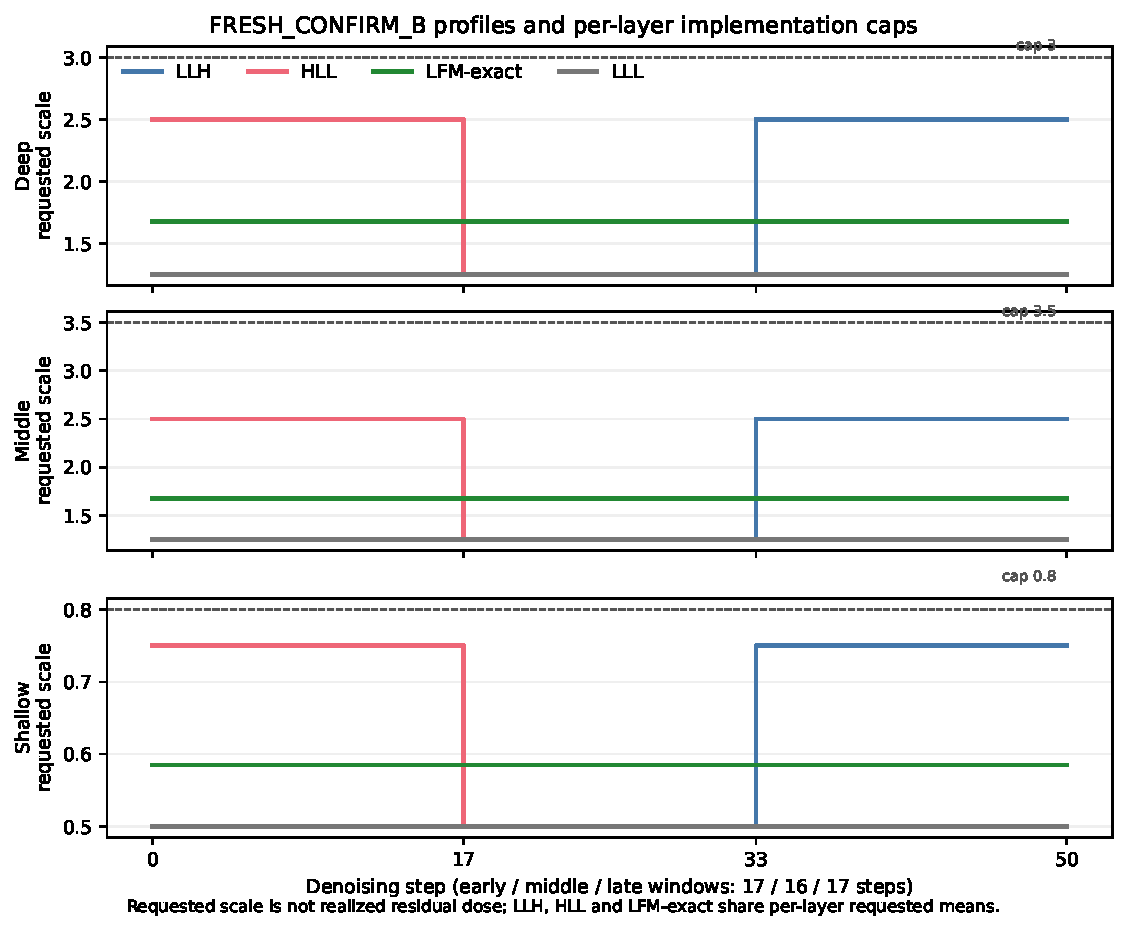
\includegraphics[width=0.84\textwidth]{b_profiles.pdf}
\caption{Requested per-layer scale profiles for the FRESH\_CONFIRM\_B comparisons. Each temporal window contains 17/16/17 steps. The dashed limits are implementation caps. LLH, HLL, and LFM-exact have the same requested per-layer means; their realized correction norms differ. LLL is the all-low reference.}
\label{fig:profiles}
\end{figure*}

\subsection{Profiles and estimands}

The primary image-space cohort is FRESH\_CONFIRM\_B: 150 objects with 30 generated conditions and 4,500 unique object-condition rows. Byte- and decoded-pixel-level cohort checks found no overlap with the earlier object cohorts. The assets are drawn from Objaverse 1.0, with source identifiers and per-model license records listed in Supplementary S10 \cite{objaverse2023}. The B registry itself is explicitly marked \texttt{RETROSPECTIVE\_LOCK\_AFTER\_PRIOR\_OUTCOME\_EXPOSURE}; therefore, although the object cohort is disjoint and its output-integrity gate passed, its comparison and analysis safeguards are not described here as prospective preregistration or blinded confirmation.

The three temporal profiles use 50 steps in early/middle/late windows of 17/16/17 steps. LLH applies (deep, middle, shallow) requested scales (1.25, 1.25, 0.50), (1.25, 1.25, 0.50), and (2.50, 2.50, 0.75) across those windows. HLL reverses the high window. LFM-exact applies the layerwise means (1.675, 1.675, 0.585) at every step. LLL is the constant low profile (1.25, 1.25, 0.50). These comparisons use the native capped wrapper. In the LLH--LFM-exact and LLH--HLL pairs, requested layer means or high-window duration are controlled as specified, but observed residual norms are not equal.

We report four contrasts separately: LLH--LFM-exact tests temporal variation at the same requested per-layer means; LLH--HLL compares early and late placement at the same high-window duration; LLH--LLL compares the profile with the all-low reference and changes total requested scale; HLL--LLL is exploratory and was computed after prior outcomes were available. The latter two are not interchangeable tests of a general early-versus-late rule.

\subsection{Cohorts and sensitivity analyses}

E1 evaluates 48 fixed objects drawn from B under generation seeds 42, 43, and 44. Seed 42 reuses the already verified B outputs; seeds 43 and 44 are new realizations. E2 evaluates a static 2\,$\times$\,2 scale factorial on the same 48 objects and three fixed seeds. It changes deep and middle scales together, varies shallow scale, and includes their factorial interaction. E1 and E2 are post-B sensitivity analyses on a reused subset, not new object-cohort confirmation or random-seed population inference.

A3b measures a bounded layer-by-window response map on B. Its corrected object-cluster Wald and GEE tests detect heterogeneity, but the planned dose calibration missed its target and the dose-adjusted three-layer model retained zero of 2,250 rows in common support. Its adjusted significance is therefore extrapolative; it does not identify a dose-independent interaction. Earlier A2 results remain discovery evidence.

A separate 24-object visual cohort was selected using ground-truth-only texture, coverage, and geometry strata before method outcomes. A native GLB evaluation uses 20 UV-supported objects, eight stored conditions, and 11 fixed unseen views per object-condition. Four objects without UV layers were excluded before baking. The GLB measurements are unlit base-color renders using each file's embedded glTF sampler under the glTF 2.0 defaults for omitted address modes \cite{gltf2020}, not a full PBR or lighting study. Cross-interface analyses are reported separately: MV-Adapter has 98 evaluable objects from 99 planned; MVDiffusion uses a separate 75-object panel with CPBlock interpolation rather than the additive geometry-residual intervention.

\subsection{Statistics}

The inferential unit is the object. For paired image-space estimates we use 10,000 object-bootstrap resamples and report two-sided percentile 95\% confidence intervals \cite{efron1993bootstrap}. The frozen correction families are Holm-adjusted separately by endpoint; bootstrap p-values at the reporting floor are shown as upper bounds. The B practical margins for LLH--LFM-exact are $\pm0.5$ dB for FG-PSNR and $\pm0.01$ for FG-LPIPS. A confidence interval within these bounds is described as practically small under those declared margins; it is not evidence of exact equivalence outside them. GLB intervals are nominal object-bootstrap intervals and are not multiplicity-adjusted. All intervals quantify object variation conditional on the tested generation protocol, not population variation over model checkpoints, samplers, or participants.

\section{Results}
\label{sec:results}

\subsection{Fresh-cohort schedule contrasts are metric- and object-dependent}

Table~\ref{tab:temporal} reports the four distinct B contrasts. LLH--LFM-exact has mean changes of +0.325 dB FG-PSNR (95\% CI [0.209, 0.446]) and -0.00460 FG-LPIPS ([-0.00563, -0.00357]). The intervals lie inside the predeclared practical margins, despite bootstrap p-values at the resolution floor after the seven-comparison endpoint-specific Holm family. This is a small average difference under the tested requested-mean match, not evidence that all temporal schedules differ meaningfully or that realized dose is matched.

For LLH--HLL, mean FG-PSNR favors LLH by +0.687 dB [0.404, 0.981], but only 45.3\% of objects favor LLH and the median difference is -0.104 dB. Thus the positive mean is heterogeneous and does not describe a typical-object PSNR gain. FG-LPIPS favors LLH on 80.7\% of objects (mean -0.01098, 95\% CI [-0.01349, -0.00851]). LLH also beats LLL on both means, but that contrast changes total requested scale as well as temporal placement. HLL--LLL is exploratory: its FG-PSNR interval crosses zero, while LPIPS favors LLL. The four comparisons do not establish the conjunction “late enhancement helps and early enhancement hurts.”

\begin{table*}[t]
\centering\small
\caption{FRESH\_CONFIRM\_B paired object-bootstrap contrasts. Deltas are first condition minus second; positive PSNR and negative LPIPS favor the first condition. HLL--LLL is exploratory.}
\label{tab:temporal}
\begin{tabular}{p{0.25\textwidth}p{0.42\textwidth}p{0.25\textwidth}}
\toprule
Contrast / endpoint & Mean change [95\% CI] & Favorable objects; Holm-adjusted p \\
\midrule
LLH minus LFM-exact, FG-PSNR (dB) & +0.325 [0.209, 0.446] & 54.0\%; p at most 0.0007 \\
LLH minus LFM-exact, FG-LPIPS & -0.00460 [-0.00563, -0.00357] & 76.0\%; p at most 0.0007 \\
LLH minus HLL, FG-PSNR (dB) & +0.687 [0.404, 0.981] & 45.3\%; p at most 0.0004; median -0.104 dB \\
LLH minus HLL, FG-LPIPS & -0.01098 [-0.01349, -0.00851] & 80.7\%; p at most 0.0004 \\
LLH minus LLL, FG-PSNR (dB) & +0.734 [0.597, 0.875] & 79.3\%; p at most 0.0004 \\
LLH minus LLL, FG-LPIPS & -0.00845 [-0.01029, -0.00659] & 82.0\%; p at most 0.0004 \\
HLL minus LLL (exploratory), FG-PSNR (dB) & +0.047 [-0.120, 0.208] & 66.0\%; p = 0.5696 \\
HLL minus LLL (exploratory), FG-LPIPS & +0.00253 [0.00155, 0.00354] & 40.0\%; p at most 0.0002 \\
\bottomrule
\end{tabular}
\end{table*}

A post-lock generic-schedule extension provides a useful comparator boundary, not a new independent confirmation. Against endpoint-matched generic linear warm-up, LLH differs by -0.037 dB FG-PSNR (95\% CI [-0.083, 0.009], Holm $p=0.115$) and +0.0011 FG-LPIPS ([0.0004, 0.0019], Holm $p=0.0024$), where lower LPIPS favors generic linear. LLH is therefore not uniformly better than a simple schedule. Other same-cohort schedule comparisons and their dose overlap limits are in the supplement and audit bundle.

\begin{figure*}[t]
\centering
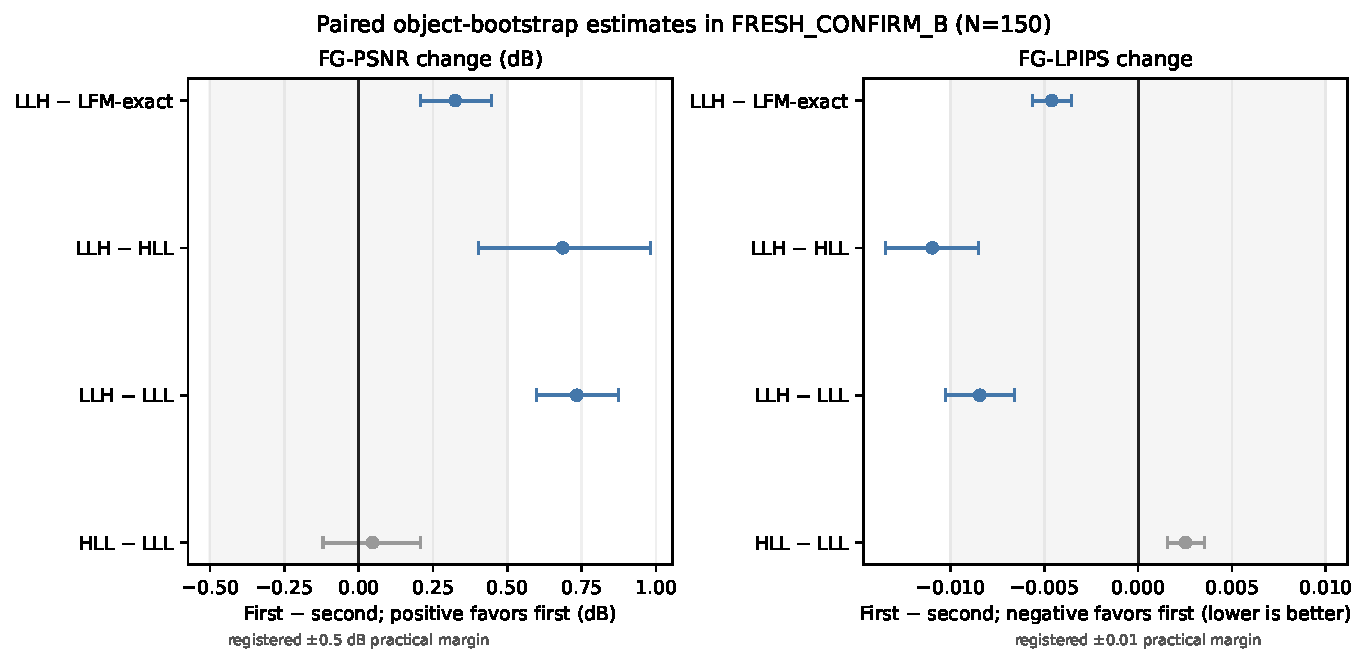
\includegraphics[width=0.92\textwidth]{b_primary_contrasts.pdf}
\caption{Paired estimates for the registered LLH contrasts and the separately marked exploratory HLL--LLL contrast. Shaded bands show the predeclared practical margins for LLH--LFM-exact. Confidence intervals describe object resampling; they do not adjust for other endpoints unless the table reports the corresponding Holm family.}
\label{fig:bcontrasts}
\end{figure*}

\subsection{Repeated realizations and static scale sensitivity}

On the reused 48-object subset, LLH--LFM-exact averages +0.329 dB FG-PSNR (95\% object-bootstrap CI [0.179, 0.497]) and -0.00391 FG-LPIPS ([-0.00549, -0.00245]) across seeds 42--44. The corresponding mean effects are about 0.58 and 0.68 times the median within-object seed range, respectively. These ratios are descriptive, and the repeated runs do not provide a new object sample or a random-seed confidence interval.

The E2 static factorial (Table~\ref{tab:factorial}) finds that raising deep and middle scales together from 1.25 to 1.675 is associated with lower FG-LPIPS and higher FG-PSNR in these 48 objects. Raising shallow scale from 0.50 to 0.80 worsens LPIPS on average, while the PSNR main effect is unresolved. The deep+middle-by-shallow interaction is detected for PSNR but not LPIPS. Deep and middle were moved together, all profiles are static over time, and realized residual dose was not matched. The PSNR interaction is also comparable in scale to the median within-object seed range; its LPIPS counterpart is much smaller. These findings support sensitivity of the specified static profiles, not a general layer-by-time mechanism.

\begin{table*}[t]
\centering\small
\caption{E2 fixed-cohort static 2\,$\times$\,2 factor effects, each object first averaged over three fixed seeds. Negative LPIPS and positive PSNR favor the higher-scale factor. Holm correction is within the three tests for each endpoint.}
\label{tab:factorial}
\begin{tabular}{llrrrl}
\toprule
Endpoint & Factor & Mean effect [95\% CI] & Favorable objects & Holm $p$ & Scope \\
\midrule
FG-LPIPS & Deep+middle & -0.00666 [-0.00887, -0.00452] & 81.2\% & 0.00030 & Deep and middle changed together \\
FG-LPIPS & Shallow & +0.00584 [0.00251, 0.00927] & 35.4\% & 0.00160 & Static scale only \\
FG-LPIPS & Interaction & -0.000147 [-0.000923, 0.000620] & 54.2\% & 0.719 & No detected interaction \\
FG-PSNR (dB) & Deep+middle & +0.544 [0.329, 0.763] & 72.9\% & 0.00030 & Static scale only \\
FG-PSNR (dB) & Shallow & -0.116 [-0.655, 0.399] & 52.1\% & 0.668 & No detected main effect \\
FG-PSNR (dB) & Interaction & +0.365 [0.243, 0.486] & 72.9\% & 0.00030 & PSNR-specific; near seed-range scale \\
\bottomrule
\end{tabular}
\end{table*}

\begin{figure*}[t]
\centering
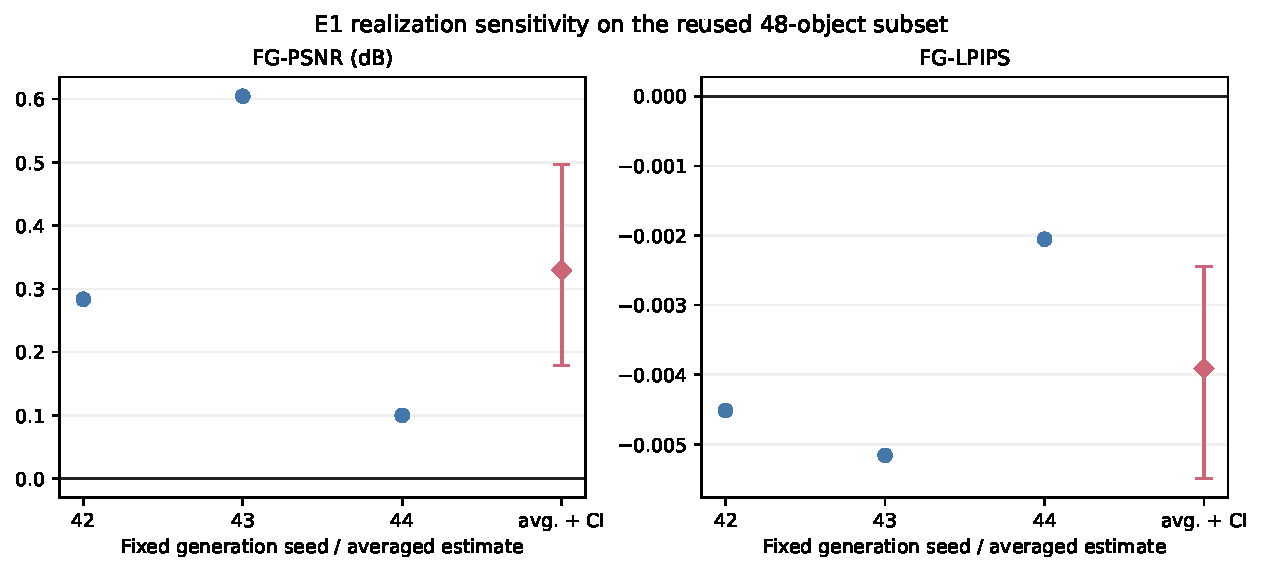
\includegraphics[width=0.48\textwidth]{e1_seed_sensitivity.pdf}\hfill
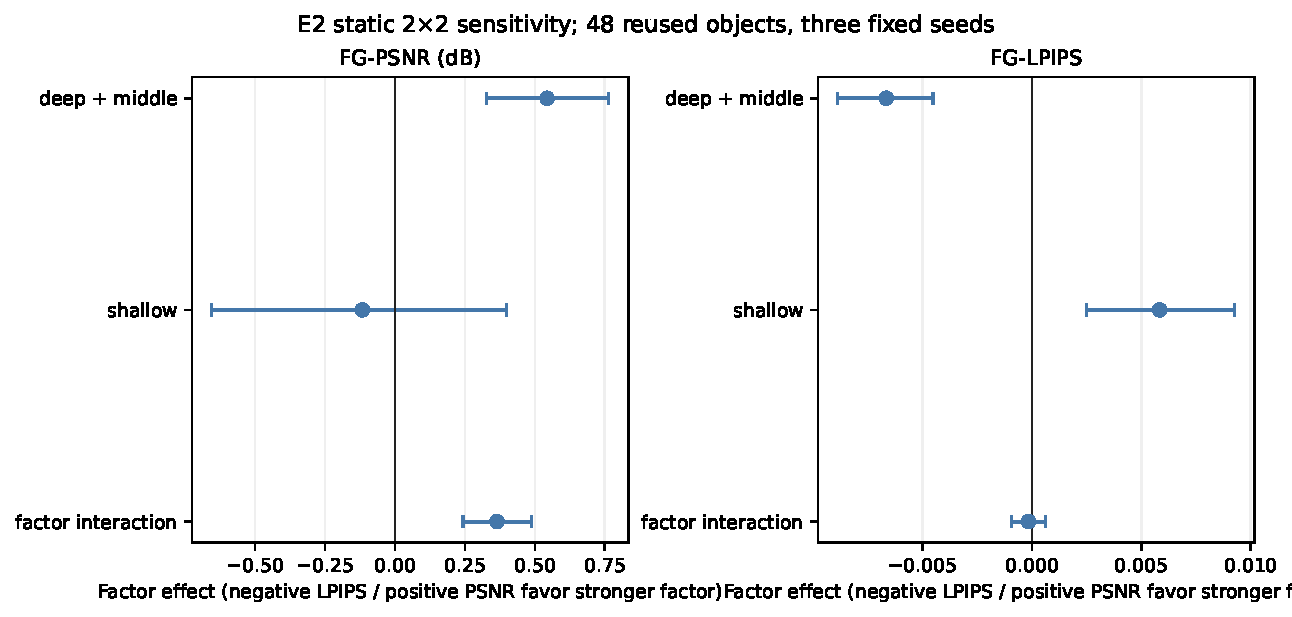
\includegraphics[width=0.48\textwidth]{e2_static_factors.pdf}
\caption{Left: E1 seed-specific means and the object-bootstrap estimate averaged across three fixed seeds. Right: E2 static factor effects on the same 48-object subset. These post-B analyses characterize realization and static-scale sensitivity; neither is an independent object-cohort confirmation.}
\label{fig:sensitivity}
\end{figure*}

\subsection{Requested scale does not identify a dose-independent interaction}

The B cap/budget accounting shows why the profile labels alone are insufficient. Native GFL, GFH, and GC3 activate the shallow cap for all 50 steps, while LLH, HLL, and LFM-exact do not activate a cap. LLH and LFM-exact have the same requested layer means and cap path but different measured correction norms. Across the 15-cell A3b bounded map, cluster-Wald and GEE tests detect layer-by-window heterogeneity, with interaction RMSE 0.000342 FG-LPIPS and 0.0205 dB FG-PSNR. However, the development dose calibration missed its target and the dose-adjusted three-layer model has no common-support rows (0/2,250 retained). Adjusted estimates thus extrapolate beyond observed overlap. We report a measurable native-dose response surface, not a dose-independent or equal-dose mechanism.

\subsection{Visual audit and stored 3D endpoints}

The GT-stratified 24-object visual audit includes the unmodified pipeline, native fixed-low, fixed-high, GC3, LFM-exact, LHL, and LLH. Manual inspection classified color/material mismatch in 18/24 panels and fine-detail loss in 21/24; it found no stable visible schedule winner. This is a descriptive author audit, not a blinded participant study. It reinforces the separation between image metrics and faithful material appearance.

The GLB-native re-render fixes the former address-mode and minification mismatch for the exact stored exports. It evaluates eight conditions on 20 UV-supported objects over 11 unseen views each (1,760 renders); no textures were rebaked. LLH--native-GFL estimates are mixed: FG-PSNR -0.422 dB (95\% CI [-1.361, 0.652]), FG-LPIPS -0.01175 ([-0.01988, -0.00564]), and CIEDE2000 \cite{sharma2005ciede} +2.563 ([-1.007, 5.893]). The LPIPS interval favors LLH; PSNR is unresolved and the CIEDE2000 point estimate favors GFL. These nominal intervals do not support an overall 3D winner. Four no-UV objects remain outside the evaluated cohort; the endpoint is unlit base-color, not full PBR. We make no seam claim because the legacy seam analyzer is not valid for the exported UV mapping. No new human preference responses were collected for LLH.

\begin{table*}[t]
\centering\small
\caption{GLB-native object-level means and the LLH--GFL endpoint differences on the supported N=20 set. Pairwise intervals are nominal and not multiplicity-adjusted.}
\label{tab:glb}
\begin{tabular}{lrrr}
\toprule
Endpoint & GFL mean & LLH mean & LLH $-$ GFL [95\% CI] \\
\midrule
FG-PSNR (dB) & 10.143 & 9.721 & -0.422 [-1.361, 0.652] \\
FG-LPIPS & 0.1390 & 0.1272 & -0.01175 [-0.01988, -0.00564] \\
CIEDE2000 & 27.34 & 29.90 & +2.563 [-1.007, 5.893] \\
\bottomrule
\end{tabular}
\end{table*}

\begin{figure*}[t]
\centering
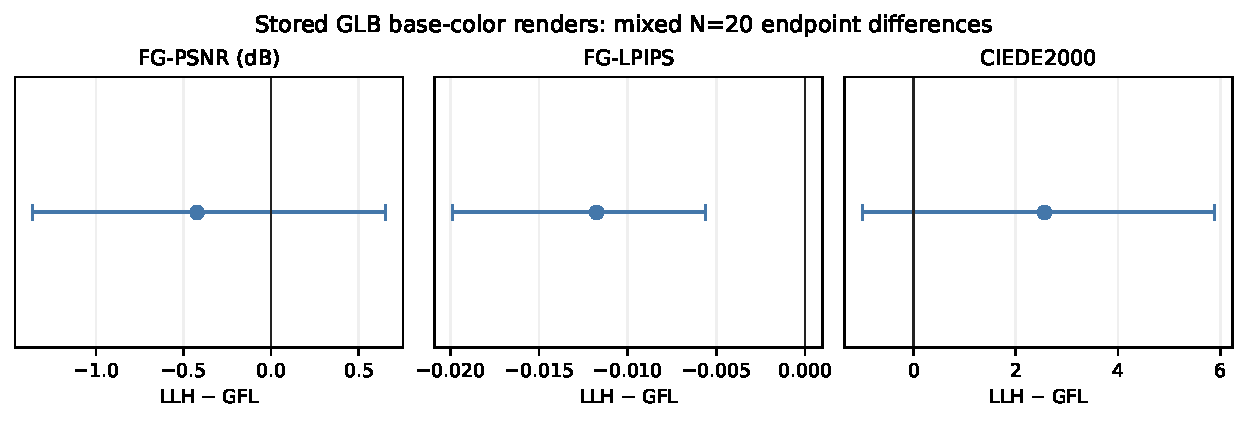
\includegraphics[width=0.82\textwidth]{glb_native_endpoints.pdf}
\caption{Stored GLB base-color endpoint differences for LLH minus native GFL. Negative LPIPS and CIEDE2000 favor LLH; positive PSNR favors LLH. The mixed estimates do not establish overall 3D superiority.}
\label{fig:glb}
\end{figure*}

\subsection{Retrospective C3 and cross-interface boundaries}

The retrospective strict-276 re-evaluation gives GC3--GFL FG-PSNR +1.208 dB (nominal object-bootstrap 95\% CI [1.117, 1.295], 259/276 objects favor GC3) and Edge-SSIM +0.00776 [0.00677, 0.00875] (233/276). The pair was not a registered primary Core-7 contrast, and the legacy input-tensor hashes and common-runner identity cannot be fully verified. A second, post-hoc analysis of the disjoint FRESH\_CONFIRM\_B objects gives GC3--GFL FG-PSNR +0.502 dB [0.342, 0.663] (100/150) and Edge-SSIM +0.00503 [0.00335, 0.00675] (105/150); all seven Core-7 mean directions favor GC3 in this pair. B had already been unblinded and this B3 pair was not registered, so this is retrospective evidence on a separate object cohort, not a prospective or registered confirmation. Against fixed-high on strict-276, GC3 loses FG-PSNR by 1.214 dB and Edge-SSIM by 0.02601, while full PSNR and full SSIM favor GC3; five of seven endpoint directions favor GFH. We therefore retire the submitted pooled +0.96 dB as an independently confirmed gain and describe these comparisons only as cohort-specific retrospective supplements. We do not transfer LLH results to C3.

On MV-Adapter (98/99 planned objects), no global interaction metric survives the exploratory four-metric correction; small shallow late-window LPIPS changes are limited to the tested intervention. On the distinct MVDiffusion interface (75 objects), CPBlock interpolation yields a structural/color versus texture-error trade-off, and the layer-wise response does not replicate. These cohorts use different control mechanisms and are not a matched architecture experiment. They support only the statement that transfer was not established across the tested interfaces.

\section{Discussion}
\label{sec:discussion}

The central result is a boundary on inference-time scale scheduling. Under a specified adapter path, caps and requested profiles produce measurable paired responses; their practical interpretation depends on endpoint, object, realization, and actual residual trace. LLH--LFM-exact is the cleanest requested-mean temporal contrast, yet its mean differences are inside the declared practical margins and its realized correction norms are not equal. LLH--HLL has metric-dependent object responses, and the early-versus-all-low exploratory comparison does not support a broad early-harm claim. A generic linear schedule also wins on the LPIPS endpoint in the same cohort. These findings argue against a unique or transferable schedule recommendation.

The evidence does not reinstate the broad novelty framing in the earlier submission. Scheduled Style Injection already studies depth/time scheduling and geometric ControlNet scale schedules. Our distinction is the audited MVPainter residual/cap path and its object-level image and stored-GLB response, not the control axes themselves. The evidence may still be judged too incremental for the target journal. Claim narrowing can make the scope accurate; it cannot guarantee methodological contribution adequacy.

Several limitations directly constrain application. The FRESH\_CONFIRM\_B registry and analysis safeguards postdate earlier outcome exposure, despite the disjoint object cohort and passing output-integrity gate. E1 and E2 reuse a fixed 48-object subset and three fixed seeds. A3b lacks dose common support. The strict-276 C3 estimate is retrospective with incomplete provenance. The GLB-native analysis covers 20 UV-supported objects and unlit base-color rendering; it does not cover four no-UV assets, full PBR appearance, or a valid seam endpoint. Visual classifications were not blinded and no new LLH human responses exist. We therefore make no human-preference, seam-quality, full-3D-fidelity, generalization, or universal-optimum claim. The earlier submitted human study concerns different scale profiles and is not transferred to LLH.

\section{Conclusion}

This study measures specified inference-time geometry-adapter scale profiles in a multi-view texture-generation pipeline. Paired object-level evidence shows a small LLH--LFM-exact difference within declared practical margins, heterogeneous LLH--HLL responses, and additional fixed-cohort sensitivity to static layer-group scales. Cap state and realized correction norms are not interchangeable with requested scale. A bounded layer-by-window interaction remains unidentified as dose-independent because the adjusted model has no common support. Stored GLB base-color endpoints are mixed, and results do not transfer uniformly to the tested adapter interfaces. The appropriate conclusion is a reproducible, pipeline-specific response characterization with explicit limits, not a general schedule law or universally preferred method.

\section*{Data and code availability}

The organized evidence package is deposited in the accompanying GitHub branch at \url{https://github.com/Blues-berry/MV-Painter/tree/codex/paper-1006-20261006/1006}. It contains audit reports, protocol and execution manifests, object-level metric tables, analysis scripts, figures, and source hashes. Large generated image and residual-trace payloads, pretrained weights, source meshes, and participant-level data are not redistributed in this package; their inclusion and licensing require a separate release decision. The human study for LLH has not been conducted, and no participant responses are included.

\section*{Declaration of competing interests}
The authors declare that they have no known competing financial interests or personal relationships that could have appeared to influence the work reported in this paper.

\begin{thebibliography}{12}
\bibitem{shao2025mvpainter}
Shao M, Xiong F, Sun Z, Xu M. MVPainter: Accurate and detailed 3D texture generation via multi-view diffusion with geometric control. arXiv:2505.12635, 2025.

\bibitem{zhang2023controlnet}
Zhang L, Rao A, Agrawala M. Adding conditional control to text-to-image diffusion models. \textit{Proceedings of the IEEE/CVF International Conference on Computer Vision}, 2023.

\bibitem{huang2025mvadapter}
Huang Z, Guo Y-C, Wang H, et al. MV-Adapter: Multi-view consistent image generation made easy. \textit{Proceedings of the IEEE/CVF International Conference on Computer Vision}, 2025, 16377--16387.

\bibitem{tang2023mvdiffusion}
Tang S, Zhang F, Chen J, Wang P, Furukawa Y. MVDiffusion: Enabling holistic multi-view image generation with correspondence-aware diffusion. \textit{Advances in Neural Information Processing Systems}, 2023.

\bibitem{kulkarni2026scheduled}
Kulkarni A S. Scheduled Style Injection: Expanding the Style-Content Pareto Frontier in Training-Free Diffusion-Based Style Transfer. In: \textit{Proceedings of the IEEE/CVF Conference on Computer Vision and Pattern Recognition Workshops (NTIRE)}, 2026. arXiv:2605.26538. \url{https://openaccess.thecvf.com/content/CVPR2026W/NTIRE/papers/Kulkarni_Scheduled_Style_Injection_Expanding_the_Style-Content_Pareto_Frontier_in_Training-Free_CVPRW_2026_paper.pdf}.

\bibitem{kynkaanniemi2024limited}
Kynk\"a\"anniemi T, Aittala M, Karras T, et al. Applying guidance in a limited interval improves sample and distribution quality in diffusion models. \textit{Advances in Neural Information Processing Systems}, 2024.

\bibitem{wang2004ssim}
Wang Z, Bovik A C, Sheikh H R, Simoncelli E P. Image quality assessment: From error visibility to structural similarity. \textit{IEEE Transactions on Image Processing}, 2004, 13(4): 600--612.

\bibitem{zhang2018lpips}
Zhang R, Isola P, Efros A A, Shechtman E, Wang O. The unreasonable effectiveness of deep features as a perceptual metric. \textit{Proceedings of the IEEE/CVF Conference on Computer Vision and Pattern Recognition}, 2018.

\bibitem{sharma2005ciede}
Sharma G, Wu W, Dalal E N. The CIEDE2000 color-difference formula: Implementation notes, supplementary test data, and mathematical observations. \textit{Color Research \& Application}, 2005, 30(1): 21--30.

\bibitem{gltf2020}
Khronos Group. glTF 2.0 specification. \url{https://registry.khronos.org/glTF/specs/2.0/}, 2020.

\bibitem{objaverse2023}
Deitke M, Schwenk D, Salvador J, Weihs L, Michel O, VanderBilt E, et al. Objaverse: A Universe of Annotated 3D Objects. \textit{Proceedings of the IEEE/CVF Conference on Computer Vision and Pattern Recognition}, 2023, 13142--13153.

\bibitem{efron1993bootstrap}
Efron B, Tibshirani R J. \textit{An Introduction to the Bootstrap}. Chapman \& Hall, 1993.
\end{thebibliography}
\end{document}
